\documentclass[12pt]{article}

\usepackage[margin=1in]{geometry}
\usepackage{amsmath}
\usepackage{amssymb}
\usepackage{amsfonts}
\usepackage{graphicx}
\graphicspath{{../Figures/}}
\usepackage{booktabs}
\usepackage{natbib}
\usepackage{setspace}
\usepackage[hidelinks]{hyperref}

% Notation
\def\ppa{\mathrm{PPA}}

\doublespacing

\title{Shot Selection or Shot Making?\\
\large The Rise in NBA Shooting Efficiency, 1997--2022}
\author{Diego Luaces\\ University of Central Florida}
\date{July 30, 2026}

\begin{document}

\maketitle

\section{Introduction}

Over the past quarter century, National Basketball Association (NBA) offenses
have transformed. Teams largely abandoned the mid-range jump shot and
redirected those attempts to the two ends of the floor: shots at the rim and
shots behind the three-point arc. Over the same period, the league became
measurably more productive with each attempt. Points per shot attempt rose
from 0.956 in the 1997--98 season to 1.063 in 2021--22, a gain of about 11
additional points per 100 attempts. Modern teams attempt roughly 88 field
goals per game, so a gain of that size is worth about 9 points per team per
game --- on the order of what separates a competitive game from a comfortable
win. The question this paper asks is not whether efficiency rose, but why.

There are two candidate explanations, and they carry different business
implications for a team. The first is \emph{shot selection}: players changed
\emph{where} they shoot, moving attempts from low-value locations to
high-value ones. If selection drives the gain, a team should invest in
strategy and analytics, because the improvement came from decisions. The
second is \emph{shot making}: players convert better \emph{from a given
location} than they used to. If making drives the gain, a team should invest
in player development, because the improvement came from skill. The two
stories imply different uses of a team's scarce resources, which is why
separating them matters.

The difficulty is that between 1997--98 and 2021--22 both forces moved at
once. The league's shot mix changed and its zone-level conversion rates
changed, and the observed rise in efficiency mixes the two together. To
untangle them, this paper constructs counterfactual seasons that never
existed: a league that shoots from the old locations with modern skill, and a
league that shoots from the new locations with old skill. Holding one force
fixed while the other moves isolates each effect, and the small remainder ---
the part earned only when both change together --- is an interaction term
with an interpretation of its own.

Using 4,678,387 field goal attempts spanning 24 NBA regular seasons, the
decomposition attributes the $+0.107$ rise in points per attempt as follows:
shot making contributes $+0.0659$ (61 percent), shot selection contributes
$+0.0451$ (42 percent), and the interaction contributes $-0.0037$ ($-3$
percent). Behind those totals sits a sharper finding. The three-point
revolution was a selection story, not a making story: the share of attempts
taken from three roughly went from one shot in six to two shots in five,
while above-the-break three-point accuracy barely moved, from 34.2 percent to
34.6 percent. The shot-making improvement happened somewhere else entirely
--- at the rim and in the paint, where conversion rose by roughly five
percentage points on a share of attempts that did not move. The negative
interaction has a clean interpretation as well: conversion improved most in
the zones the league was abandoning, and skill gains on shots a league no
longer takes are worth less.

The remainder of this paper is organized as follows. Section 2 places the
question in the sports analytics literature. Section 3 presents the
accounting framework and the counterfactual decomposition, including a
simplified two-shot example that builds the intuition. Section 4 describes
the dataset and the construction of the season and zone variables. Section 5
presents the empirical results. Section 6 concludes and outlines limitations.

\section{Related Literature}

Quantitative evaluation of basketball offenses begins from the observation
that possessions, not minutes or games, are the natural unit of production.
\citet{oliver2004} organizes offensive analysis around points per possession,
and \citet{kubatko2007} formalize the possession-based accounting that has
since become standard; \citet{alamar2013} surveys how these tools entered
front-office decision-making. The transformation of NBA shot selection itself
is well documented: \citet{goldsberry2019} traces the league-wide migration of
attempts away from the mid-range and toward the rim and the three-point line,
popularly called the ``three-point revolution.'' That literature establishes
\emph{that} the shot map changed; it is less precise about how much of the
resulting efficiency gain the new map explains, as opposed to players simply
converting better.

Separating a change in composition from a change in rates is a classical
measurement problem, and the method used here follows the logic of
standardization decompositions of exactly this kind \citep{kitagawa1955}:
hold one component at its baseline value, let the other take its later value,
and attribute the difference. This paper applies that accounting to a
quarter century of NBA shot-level data and reports not only the aggregate
split between selection and making, but the zone-by-zone anatomy of each
effect, which is where the more surprising results live.

\section{Methodology}

\subsection{Shooting as a portfolio problem}

It is useful to think of a team's shot attempts as an investment portfolio in
which each court location is an asset. An asset's return is its make rate
times its point value, measured in points per attempt. A team can raise its
overall return in exactly two ways: it can shift weight toward assets that
already pay more, which is selection, or it can raise the return an asset
itself pays by converting it more often, which is making. A return is
therefore not a fixed label on a location --- making can move it. An offense
maximizing expected points should, at the margin, equalize returns across the
locations it uses; large and persistent gaps between locations are the
economic signal that a better allocation exists.

\subsection{The points-per-attempt identity}

Let $z$ index court zones and $t$ index seasons. League points per attempt in
season $t$ is a weighted average over zones:
\begin{equation}
\ppa_t \;=\; \sum_{z} s_{zt}\, p_{zt}\, v_{z},
\label{eq:identity}
\end{equation}
where $s_{zt}$ is the share of attempts taken from zone $z$ (the shot
\emph{mix}), $p_{zt}$ is the make rate in zone $z$ (the \emph{conversion}
skill), and $v_z$ is the point value of the shot, 2 or 3. Equation
(\ref{eq:identity}) is an identity, not a model: it holds exactly in every
season by construction. \emph{Selection} changes the shares $s_{zt}$ holding
conversion fixed; \emph{making} changes the rates $p_{zt}$ holding the mix
fixed. Between the two endpoint seasons both moved at once, and the
decomposition untangles them with counterfactuals.

\subsection{Counterfactual seasons and the decomposition}

Write 97 for the 1997--98 season and 21 for 2021--22. Four numbers are
needed, two real and two imaginary:
\begin{align*}
A &: \text{1997 mix, 1997 rates} \qquad \text{(actual 1997--98)}\\
D &: \text{2021 mix, 2021 rates} \qquad \text{(actual 2021--22)}\\
B &: \text{1997 mix, 2021 rates} \qquad \text{(counterfactual)}\\
C &: \text{2021 mix, 1997 rates} \qquad \text{(counterfactual)}
\end{align*}
$B$ asks: what would the league have scored if players shot from the old
places with modern skill? $C$ asks: what if players shot from the new places
with old skill? Neither league ever existed; both are built from the data by
combining the observed shares of one season with the observed rates of the
other inside equation (\ref{eq:identity}).

Both effects are measured against the 1997 baseline:
\begin{align}
\text{Making}    &= B - A = \sum_z s_{z,97}\,\left(p_{z,21}-p_{z,97}\right) v_z,
\label{eq:making}\\
\text{Selection} &= C - A = \sum_z \left(s_{z,21}-s_{z,97}\right) p_{z,97}\, v_z,
\label{eq:selection}\\
\text{Interaction} &= (D-A) - \text{Making} - \text{Selection}.
\label{eq:interaction}
\end{align}
The making effect in equation (\ref{eq:making}) prices the change in
conversion rates using the old shot mix as weights; the selection effect in
equation (\ref{eq:selection}) prices the change in the mix using the old
conversion rates. The interaction in equation (\ref{eq:interaction}) is the
piece of the total change earned only when both move together. The three
terms sum exactly to the total change $D-A$, so nothing is lost and nothing
is double counted. Because equations (\ref{eq:making}) and
(\ref{eq:selection}) are sums over zones, each aggregate effect can also be
reported zone by zone, which Section 5 exploits.

\subsection{Building the intuition: a two-shot league}

Before applying the decomposition to seven zones and 24 seasons, it helps to
see it work in a league with only two shot types, twos and threes, and two
seasons with round numbers chosen to resemble the real endpoints
(Table~\ref{tab:twoshotinputs}).

\begin{table}[ht]
\begin{spacing}{1.0}
\centering
\caption{A simplified two-shot league.}
\label{tab:twoshotinputs}
\begin{tabular}{lcc}
\toprule
                  & 1997 & 2022 \\
\midrule
Share of twos     & 80\% & 60\% \\
Share of threes   & 20\% & 40\% \\
Make rate, twos   & 48\% & 52\% \\
Make rate, threes & 33\% & 36\% \\
\bottomrule
\end{tabular}
\end{spacing}
\end{table}

The two actual seasons evaluate to
\begin{align*}
\ppa_{1997} &= (.80)(.48)(2) + (.20)(.33)(3) = .768 + .198 = 0.966,\\
\ppa_{2022} &= (.60)(.52)(2) + (.40)(.36)(3) = .624 + .432 = 1.056,
\end{align*}
a total improvement of $1.056 - 0.966 = 0.090$ points per attempt.

Selection alone applies the 2022 mix to 1997 skill:
\begin{equation*}
(.60)(.48)(2) + (.40)(.33)(3) = 0.972,
\end{equation*}
which against the baseline of 0.966 means the new shot diet by itself adds
$+0.006$. Making alone applies 2022 skill to the 1997 mix:
\begin{equation*}
(.80)(.52)(2) + (.20)(.36)(3) = 1.048,
\end{equation*}
so better skill by itself adds $+0.082$. Selection plus making is
$0.006 + 0.082 = 0.088$, but the total change was $0.090$. The missing
$0.002$ is the interaction: improved three-point skill is worth more when
threes are a bigger share of the diet. The lesson of the toy league carries
directly into the real data: skill gains are graded on the shots a league
actually takes. In this example the interaction is positive because skill
improved in the shot that was growing; Section 5 shows that in the real data
the sign flips, and why.

\section{Data}

\subsection{Dataset description}

The empirical analysis uses the NBA shot dataset provided for this course:
4,678,387 field goal attempts covering the seasons 1997--98 through 2021--22.
Each observation is a single shot attempt and records the shot's location on
the court, its distance from the basket, its assigned court zone, the shot
type (two- or three-point attempt), and the outcome (made or missed). The
2002--03 season is absent from the source data by design, leaving 24 seasons.
Every quantity in this paper --- shares, make rates, and all counterfactuals
--- is computed from this file alone; no external data are required.

The analysis is restricted to regular season games, verified from the game
identifiers as described next, so that changes in the shot landscape are not
confounded by the different competitive conditions of playoff basketball.

\subsection{Assigning shots to seasons}

Assigning each shot to the correct season is less trivial than it appears,
because the natural approach --- filtering on calendar dates --- fails in the
pandemic years. The 2019--20 season finished in October 2020, and the
2020--21 season began in December rather than October, so date windows that
work for two decades silently misclassify two seasons.

The solution used here decodes the season directly from the game identifier,
whose structure encodes it: the third digit gives the game type, with a value
of 2 denoting a regular season game, and digits four and five give the
starting year of the season. Season assignment built this way is immune to
calendar disruptions. Applying the decoding to the full file confirms that
every one of the 4,678,387 rows corresponds to a regular season game, and it
assigns each row to its season without reference to the game date.

\subsection{Zones and the endpoint seasons}

Shots are grouped into the dataset's seven basic zones; the two corner-three
zones behave nearly identically and are reported combined, giving six rows:
Restricted Area, Paint (non-restricted area), Mid-Range, Above the Break 3,
Corner 3, and Backcourt. Table~\ref{tab:endpoints} reports each zone's share
of attempts and make rate in the two endpoint seasons; these twenty-four
numbers, together with the point values, are the entire input to the
decomposition.

\begin{table}[ht]
\begin{spacing}{1.0}
\centering
\caption{Shot mix and make rates by zone, endpoint seasons.}
\label{tab:endpoints}
\begin{tabular}{lcccc}
\toprule
 & \multicolumn{2}{c}{Share of attempts} & \multicolumn{2}{c}{Make rate} \\
Zone & 1997--98 & 2021--22 & 1997--98 & 2021--22 \\
\midrule
Restricted Area   & 33.3\% & 29.1\% & 60.2\% & 65.3\% \\
Paint (non-RA)    & 14.1\% & 18.3\% & 37.0\% & 42.8\% \\
Mid-Range         & 36.9\% & 12.8\% & 38.9\% & 40.7\% \\
Above the Break 3 & 12.7\% & 29.7\% & 34.2\% & 34.6\% \\
Corner 3          &  2.9\% &  9.9\% & 37.2\% & 38.3\% \\
Backcourt         &  0.1\% &  0.2\% &  4.9\% &  2.5\% \\
\bottomrule
\end{tabular}
\end{spacing}
\end{table}

\section{Results and Discussion}

\subsection{The two headline trends}

Figure~\ref{fig:headline} plots the two series that motivate the paper.
League points per attempt rises from 0.956 in 1997--98 to 1.063 in 2021--22,
while the share of attempts taken from three climbs from roughly one shot in
six to two shots in five. This trade of long twos for threes is what is
commonly called the three-point revolution. The two series clearly move
together; the decomposition below asks how much of the first the second
actually explains.

\begin{figure}[ht]
\centering
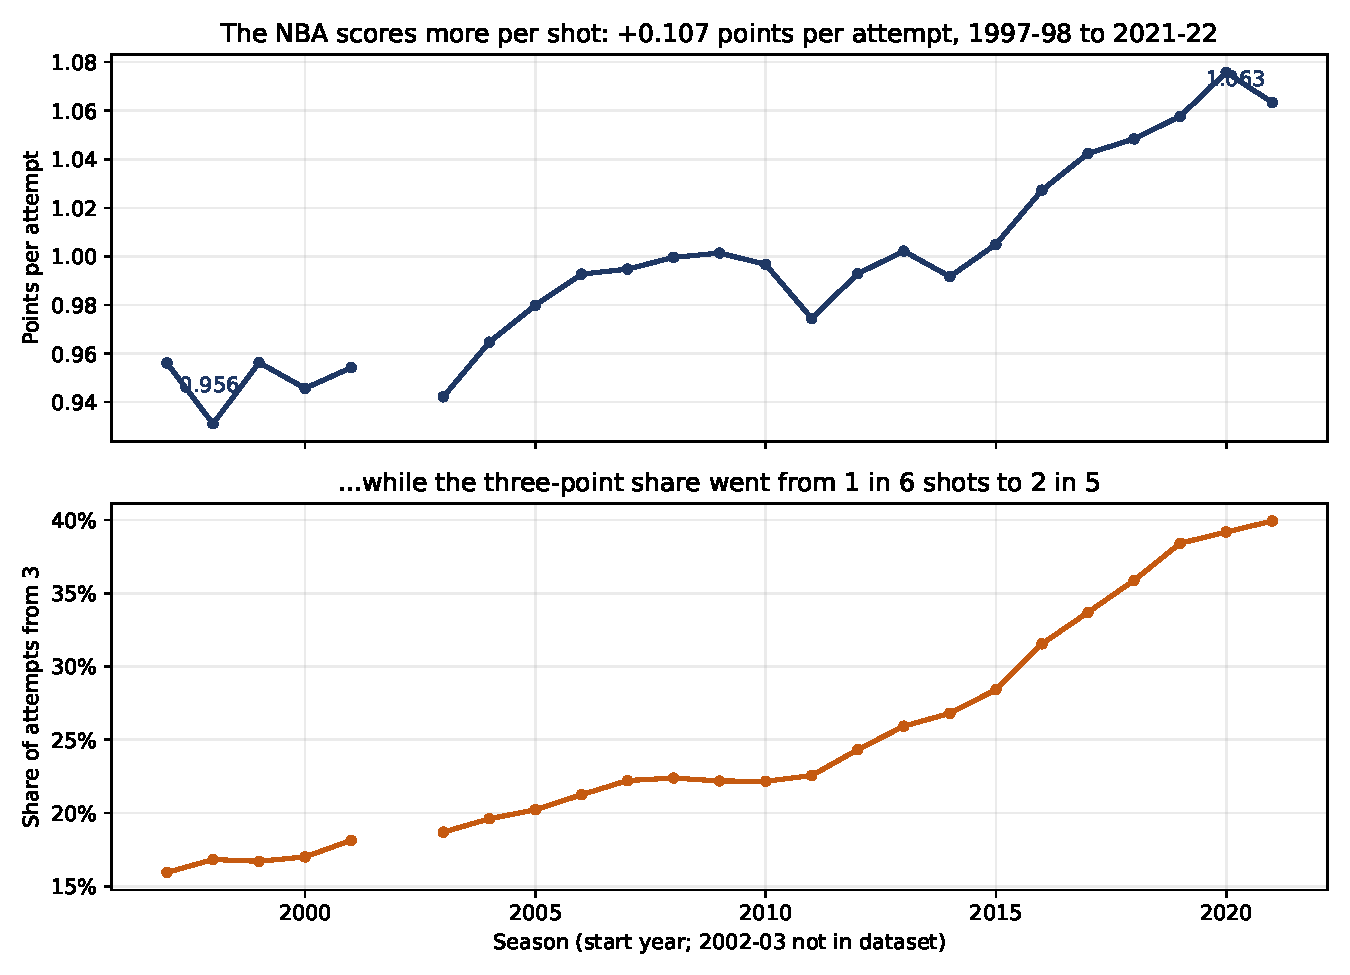
\includegraphics[width=0.85\textwidth]{Figure1.pdf}
\caption{League points per attempt (top) and the three-point share of
attempts (bottom), 1997--98 through 2021--22. The gap in each series is the
missing 2002--03 season.}
\label{fig:headline}
\end{figure}

\subsection{Where the shots went}

Figure~\ref{fig:mix} shows the full 24-season evolution of the shot mix by
zone, and Figure~\ref{fig:dumbbell} compares the endpoint seasons directly.
The mid-range collapsed from 36.9 percent of all attempts to 12.8 percent.
Above-the-break threes rose from 12.7 percent to 29.7 percent, and corner
threes more than tripled, from 2.9 percent to 9.9 percent. Meanwhile the rim
fell slightly and the paint grew by almost the same amount, leaving the total
close-range share essentially unchanged at 47 percent in both endpoint
seasons. The reallocation, in other words, was almost entirely a
mid-range-to-three trade; the inside game kept its share of the portfolio
throughout.

\begin{figure}[ht]
\centering
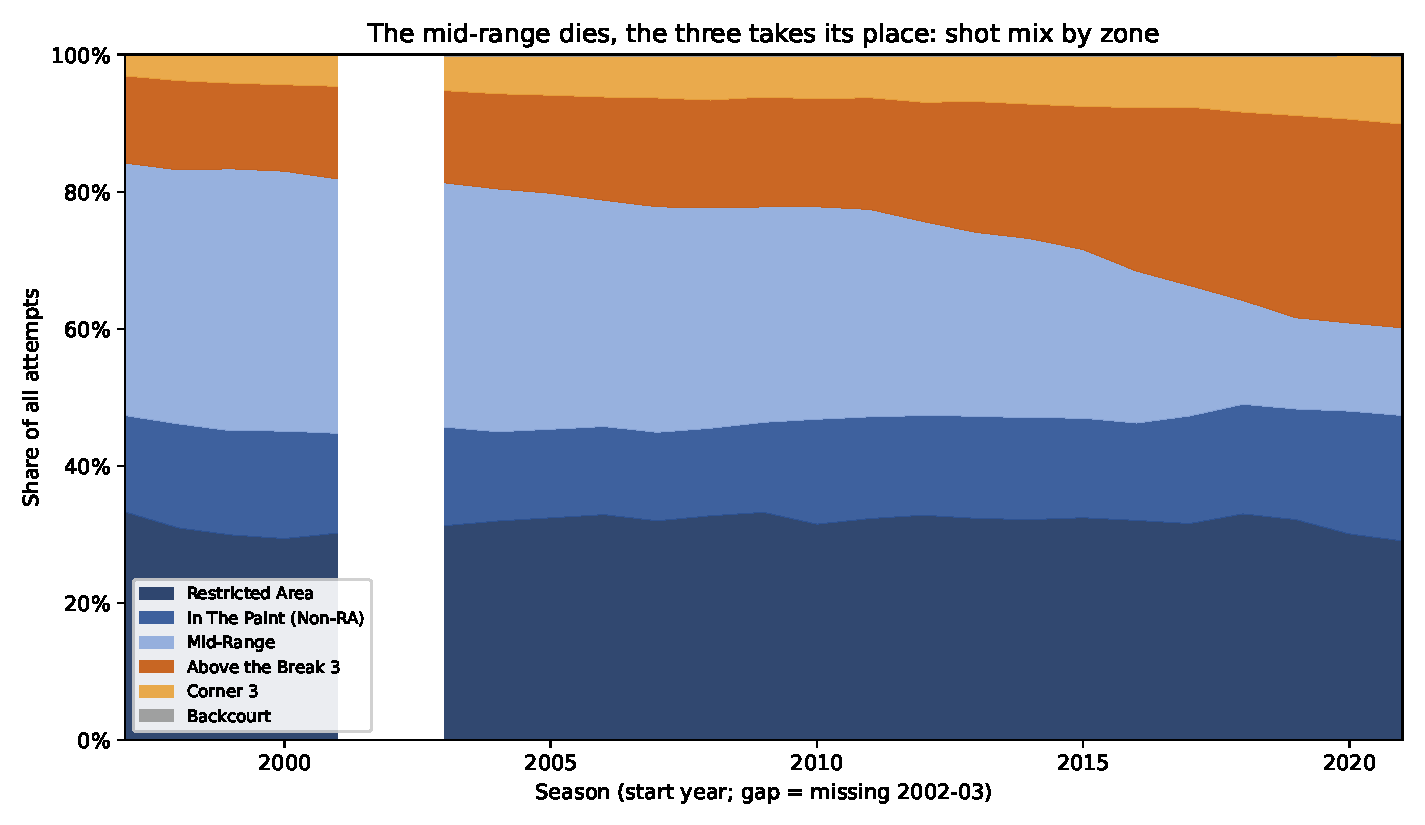
\includegraphics[width=0.95\textwidth]{Figure2.pdf}
\caption{Share of all attempts by zone across 24 seasons. The mid-range
declines steadily while the two three-point zones absorb its share; the gap
marks the missing 2002--03 season.}
\label{fig:mix}
\end{figure}

\begin{figure}[ht]
\centering
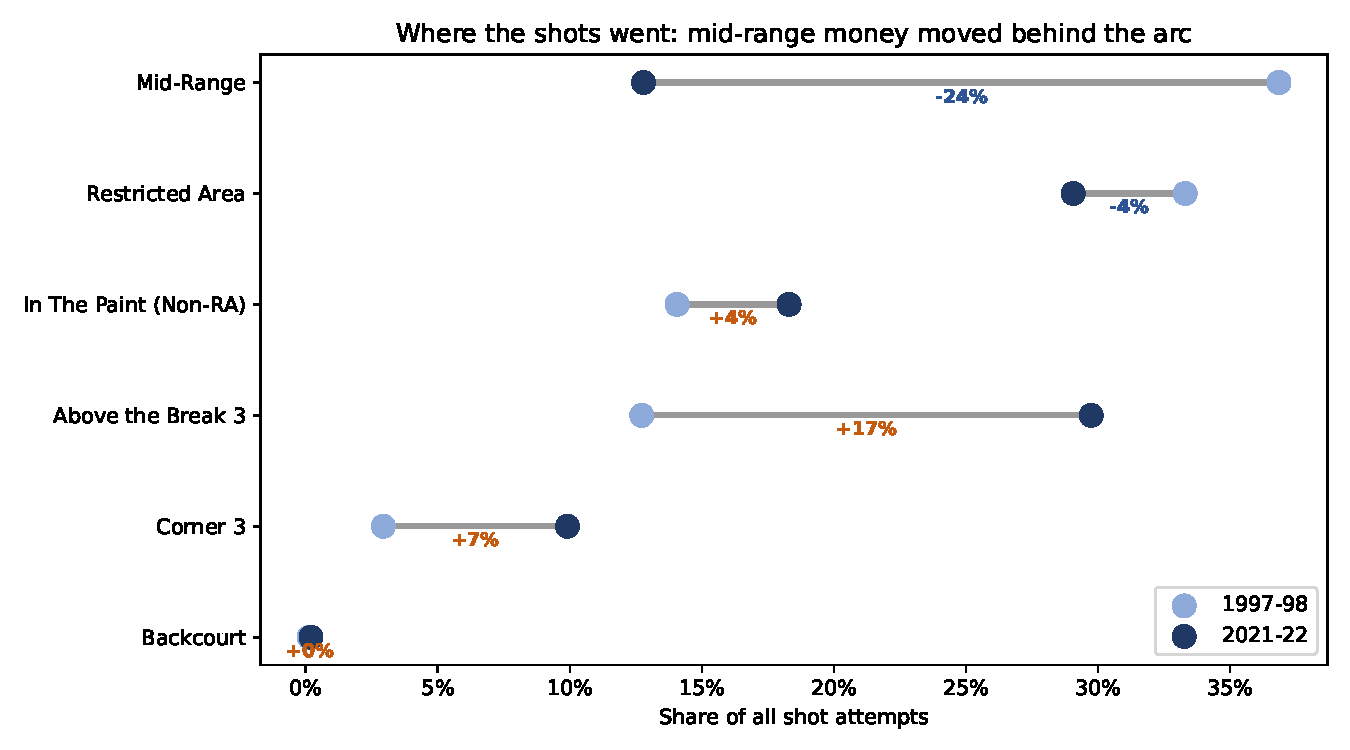
\includegraphics[width=0.95\textwidth]{Figure3.pdf}
\caption{Zone shares of attempts in 1997--98 versus 2021--22. Mid-range
money moved behind the arc.}
\label{fig:dumbbell}
\end{figure}

The economics of the trade are visible in the 1997 returns themselves. At
1997--98 conversion rates, a mid-range attempt was worth
$0.389 \times 2 = 0.78$ points while an above-the-break three was worth
$0.342 \times 3 = 1.03$ points. The league moved volume from the cheapest
shot on the floor to a considerably more valuable one --- exactly the
reallocation the portfolio logic of Section 3.1 prescribes when returns
across assets are far from equalized. Figure~\ref{fig:density} shows the
same migration spatially.

\begin{figure}[ht]
\centering
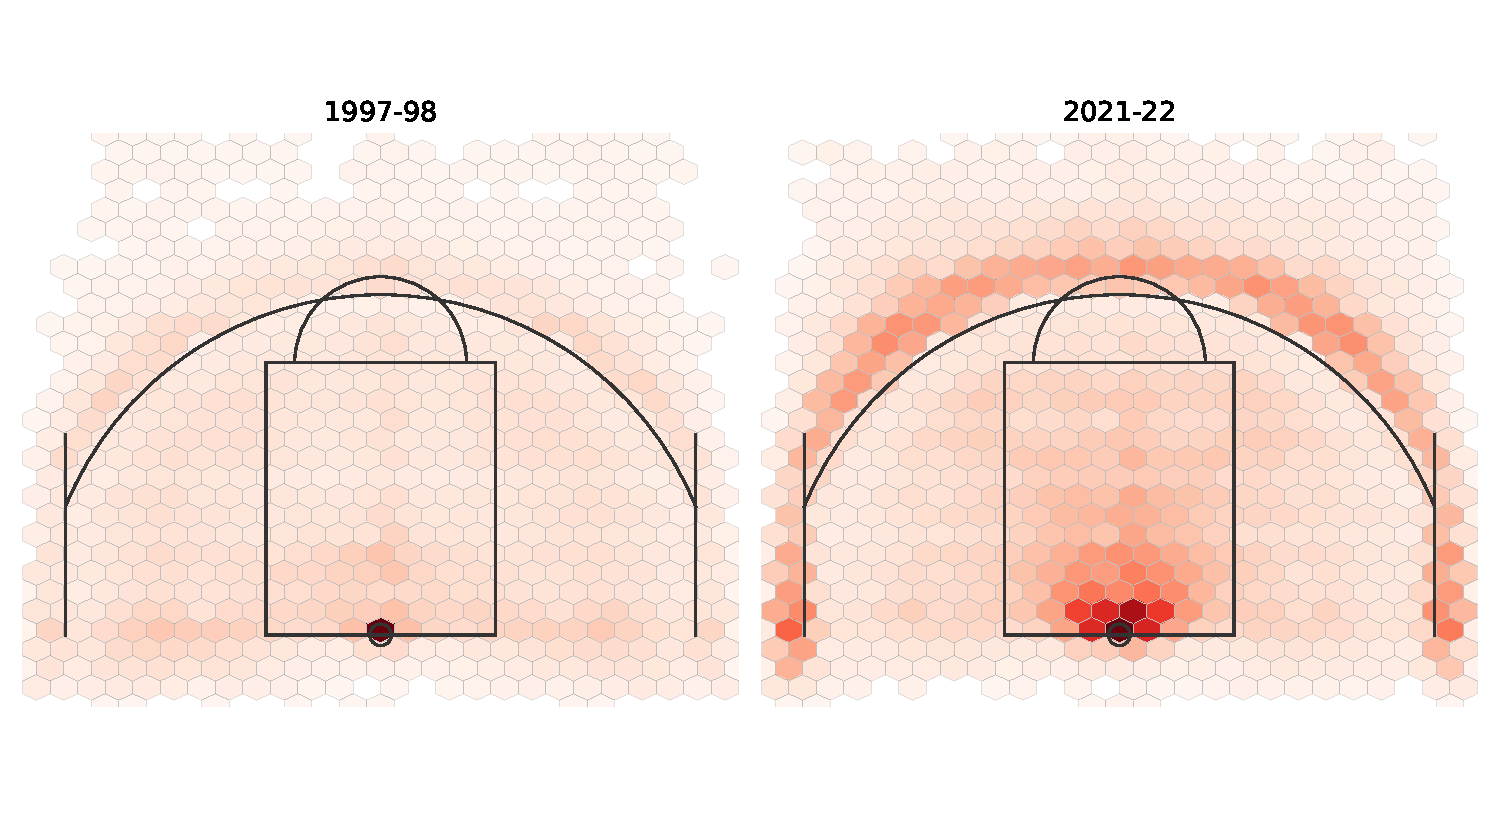
\includegraphics[width=0.85\textwidth]{Figure4.pdf}
\caption{Shot density on the court, 1997--98 (left) versus 2021--22 (right).}
\label{fig:density}
\end{figure}

\subsection{The surprise in the make rates}

Figure~\ref{fig:makerates} plots make rates by zone across all 24 seasons,
and it contains the result that reframes the three-point revolution.
Above-the-break three-point accuracy was 34.2 percent in 1997--98 and 34.6
percent in 2021--22. Twenty-five years of teams reorganizing their offenses
around the three-point shot, and players are not meaningfully better at
making threes. Corner-three accuracy moved similarly little, from 37.2 to
38.3 percent.

Where conversion did improve is inside: the restricted area rose from 60.2
percent to 65.3 percent, and the paint from 37.0 percent to 42.8 percent.
The shot-making story of the modern NBA happened at the rim and in the paint,
not behind the arc. Notably, the improvement in finishing is not a dunk
artifact: the dunk's share of attempts barely moved over the period and dunk
accuracy actually fell, so the gain reflects better finishing on the harder
close-range attempts --- layups, floaters, and finishing through contact.

\begin{figure}[ht]
\centering
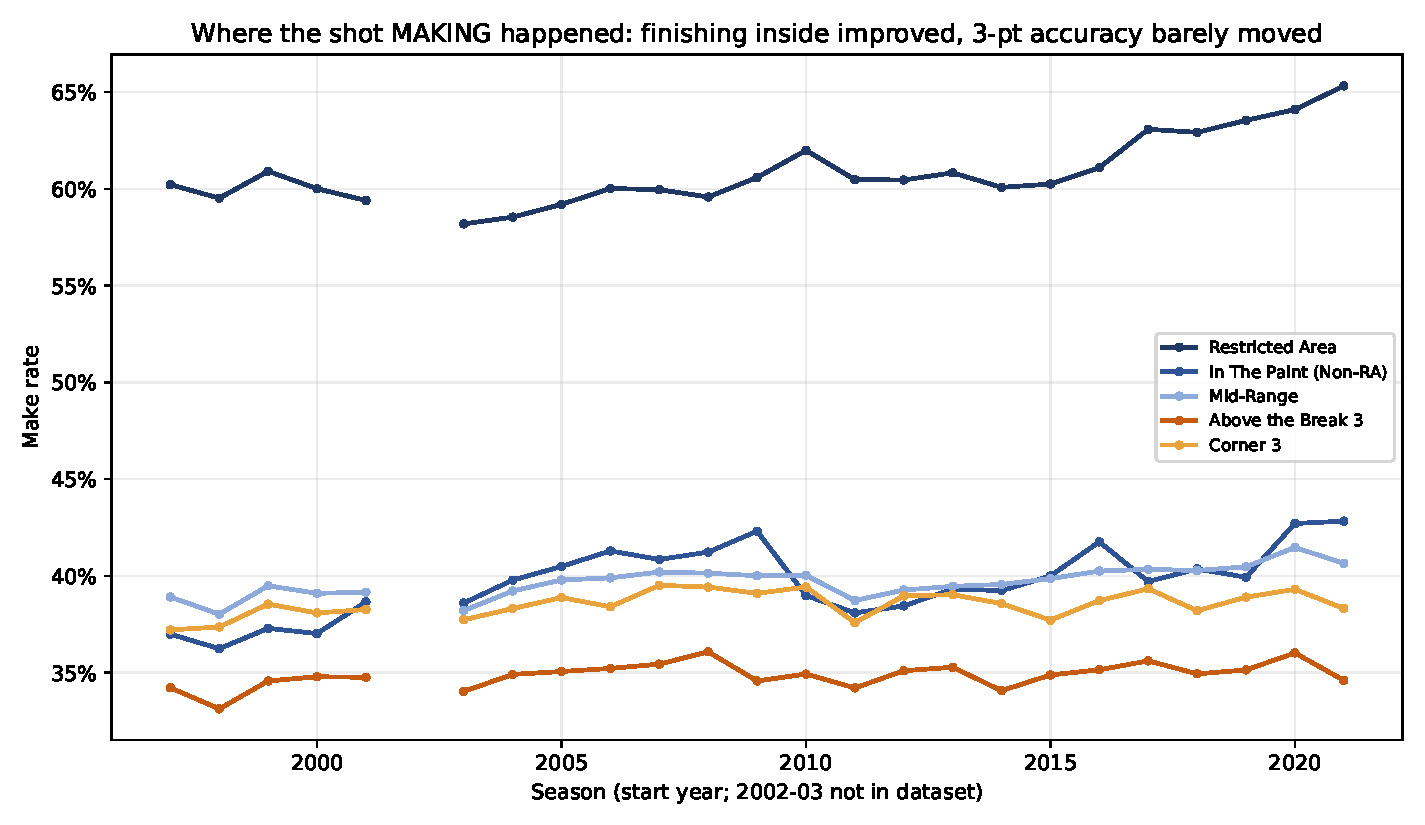
\includegraphics[width=0.95\textwidth]{Figure5.pdf}
\caption{Make rates by zone across 24 seasons. Finishing inside improved;
three-point accuracy barely moved.}
\label{fig:makerates}
\end{figure}

\subsection{Decomposition results}

Table~\ref{tab:decomp} reports the decomposition of equations
(\ref{eq:making})--(\ref{eq:interaction}) applied to the endpoint seasons;
Figure~\ref{fig:waterfall} shows it as a bridge.

\begin{table}[ht]
\begin{spacing}{1.0}
\centering
\caption{Decomposition of the change in points per attempt, 1997--98 to
2021--22.}
\label{tab:decomp}
\begin{tabular}{lr}
\toprule
Points per attempt, 1997--98 (actual)   & 0.956 \\
Points per attempt, 2021--22 (actual)   & 1.063 \\
\midrule
Total change                            & $+0.1073$ \\
\midrule
Shot making (2021 rates on 1997 mix)    & $+0.0659$ \enspace (61\%) \\
Shot selection (1997 rates on 2021 mix) & $+0.0451$ \enspace (42\%) \\
Interaction                             & $-0.0037$ \enspace ($-3\%$) \\
\bottomrule
\end{tabular}
\end{spacing}
\end{table}

\begin{figure}[ht]
\centering
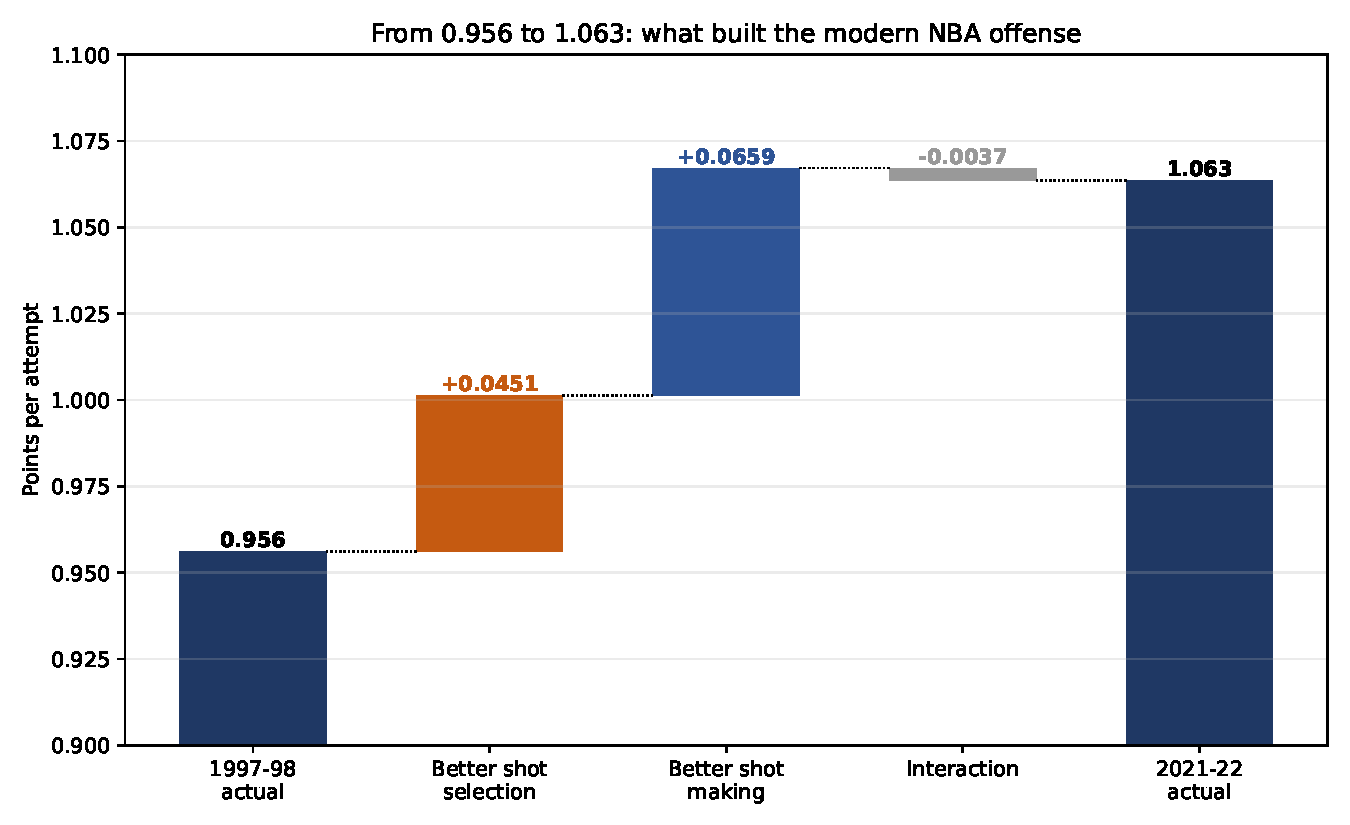
\includegraphics[width=0.9\textwidth]{Figure6.pdf}
\caption{The change in points per attempt as four steps: the 1997--98
baseline, the selection effect, the making effect, the interaction, and the
2021--22 actual.}
\label{fig:waterfall}
\end{figure}

Shot making explains 61 percent of the efficiency gain and shot selection 42
percent, with a small negative interaction closing the identity. Both forces
are large; neither story is sufficient on its own. But the aggregate split
understates how different the two effects are, because they operate in
almost entirely different places on the floor.
Table~\ref{tab:zonecontrib} breaks each effect into its zone-level
contributions from equations (\ref{eq:making}) and (\ref{eq:selection}).

\begin{table}[ht]
\begin{spacing}{1.0}
\centering
\caption{Zone-level contributions to each effect, in points per attempt.}
\label{tab:zonecontrib}
\begin{tabular}{lrr}
\toprule
Zone & Selection part & Making part \\
\midrule
Mid-Range         & $-0.188$ & $+0.013$ \\
Restricted Area   & $-0.051$ & $+0.034$ \\
Paint (non-RA)    & $+0.031$ & $+0.016$ \\
Above the Break 3 & $+0.175$ & $+0.002$ \\
Corner 3 (both)   & $+0.078$ & $+0.001$ \\
\bottomrule
\end{tabular}
\end{spacing}
\end{table}

The selection effect is a mid-range-to-arc story: the collapse of the
mid-range subtracts $0.188$ points per attempt on its own, and the growth of
the two three-point zones adds $0.175 + 0.078 = 0.253$, with smaller
movements inside netting the total to $+0.045$. The making effect is an
inside story: of its $+0.066$ total, $0.034$ comes from the restricted area
and $0.016$ from the paint, while the three-point zones together contribute
essentially nothing ($+0.003$). Selection happened at the arc; making
happened at the rim.

\subsection{Why the interaction is negative}

In the two-shot league of Section 3.4 the interaction was positive: skill
improved in the shot whose share was growing, so the two changes reinforced
each other. In the real data the interaction is negative, $-0.0037$, and the
zone anatomy explains why. Conversion improved most in zones the league was
\emph{abandoning} --- mid-range accuracy rose from 38.9 to 40.7 percent while
the league walked away from mid-range shots --- and barely improved in the
zone whose share grew most. Skill gains on shots a league no longer takes are
worth less than the same gains would have been under the old mix. The
interaction term is small, but its sign is informative: the league's two
improvements happened in opposite places.

\subsection{Implications for team investment}

The zone anatomy turns the decomposition into concrete guidance for how a
team should spend, because it identifies which improvements were decisions
and which were skills.

The three-pointer was a decision, not a skill. Teams went from 16 percent of
their shots behind the arc to 40 percent, while accuracy over those same 25
years moved from 34.2 to 34.6 percent. The league did not get better at
shooting threes; it got better at choosing them. The implication is to stop
paying for three-point accuracy as if it were a trainable, scalable input ---
twenty-five years, thirty teams, and every shooting coach in the sport moved
league accuracy less than half a percentage point --- and to pay instead for
three-point \emph{volume}: spacing, ball movement, and quick release,
anything that turns a contested three into an open one. The box score cannot
tell a contested three from an open one; the scoreboard can.

Finishing inside was a skill, not a decision. The combined rim-and-paint
share of attempts never moved --- 47 percent in both endpoint seasons ---
while its combined make rate rose from 53.3 percent to 56.6 percent, and not
through dunks. That is the one conversion skill in this data that measurably
improved, so it is the one worth paying player-development resources to
acquire: floaters, control near the basket, finishing through contact.
Finally, the mid-range is best left alone. It is down to one shot in eight,
and the attempts that survive belong disproportionately to players who are
genuinely good from there --- which is part of why the zone's measured
accuracy rose even as its volume collapsed.

There is also a broader lesson in the selection effect itself. The efficiency
gain of this era came from being early to a shot the league had underpriced:
in 1997 an above-the-break three returned 1.03 points per attempt against
0.78 for a mid-range two, and the teams that moved first collected that gap.
That particular trade is now closed --- every team shoots threes, and the
mid-range is nearly empty --- so the transferable skill is not ``shoot more
threes.'' It is finding the next underpriced shot before everyone else does,
and points per attempt by location, combined with counterfactuals that hold
one force fixed, is precisely the toolkit for finding it.

\section{Conclusion}

This paper asked how much of the NBA's quarter-century rise in shooting
efficiency came from shot selection and how much from shot making. Using an
exact decomposition of the points-per-attempt identity over 4,678,387 shot
attempts and 24 seasons, the answer is that making explains 61 percent of the
$+0.107$ gain, selection 42 percent, and a small negative interaction the
remainder. As Section 5 shows, the two forces are not just separable in size
but in location: selection happened at the arc, making happened at the rim,
and a team invests in the two very differently.

Three limitations qualify these results. First, shot selection is endogenous
to defensive pressure: defenses adapted over the same period, so the
decomposition is descriptive accounting rather than a causal estimate of what
any single team would gain by changing its mix. Second, zone-level rates can
mask changes within zones. The mid-range shots that survived the collapse are
the ones worth taking, so some of that zone's rising accuracy reflects better
shot quality within the zone rather than better shooting --- a composition
effect operating one level below the decomposition. Third, everything here is
a league-wide average: team and player heterogeneity is deliberately set
aside, and the aggregate split need not describe any individual team's
history. Extending the decomposition to the team level, where selection and
making can be compared across organizations, is a natural direction for
future work.

\bibliographystyle{plainnat}
\begin{spacing}{1.0}
\bibliography{references}
\end{spacing}

\end{document}
